\section{邻域、区域与函数}

本节介绍二元函数微积分的基础概念。

本节要点:
\begin{itemize}
    \item 掌握邻域的概念;
    \item 理解点集的各个概念;
    \item 熟悉二元函数的定义。
\end{itemize}

%============================================================
\subsection{邻域}

\begin{definition}[邻域]
设矢量$\boldsymbol{p}_0\in \mathbb{R} ^2$,对于$\delta >0$,所有符合$\left\| \boldsymbol{p}-\boldsymbol{p}_0 \right\| <\delta $的矢量$\boldsymbol{p}$的集合,称为{\bf $\boldsymbol{p}_0$的$\delta $邻域},记作$U\left( \boldsymbol{p}_0,\delta \right) $,若点$\boldsymbol{p}_0$不包含在邻域内,称该集合为{\bf $\boldsymbol{p}_0$的空心$\delta $邻域},记作$U\left( \boldsymbol{\hat{p}}_0,\delta \right) $,即:
\begin{align*}
&U\left( \boldsymbol{p}_0,\delta \right) :=\left\{ \boldsymbol{p}\in \mathbb{R} ^2 \middle| \left\| \boldsymbol{p}-\boldsymbol{p}_0 \right\| <\delta \right\} \\
&U\left( \boldsymbol{\hat{p}}_0,\delta \right) :=\left\{ \boldsymbol{p}\in \mathbb{R} ^2 \middle| 0<\left\| \boldsymbol{p}-\boldsymbol{p}_0 \right\| <\delta \right\}
\end{align*}
\end{definition}

邻域的定义和一元函数中的概念一样,定义了以某点为中心的一个范围。
几何上,二元函数的邻域是一个“面”,三元函数中是一个“球”。

%============================================================
\subsection{点、集和区域}

\begin{definition}

设点集$D$中的点$\boldsymbol{p}_0$,若存在$\boldsymbol{p}_0$的某个邻域$U\left( \boldsymbol{p}_0,\delta \right) \subset D$,称点$\boldsymbol{p}_0$为$D$的{\bf 内点}。
如果点$\boldsymbol{p}_0$的任一邻域中,既有属于$D$的点,也有不属于$D$的点,称点$\boldsymbol{p}_0$为$D$的{\bf 边界点}。
内点和边界点又称为{\bf 聚点}。
$D$的边界点的集合称为$D$的{\bf 边界}。
注意,边界点既可以属于$D$(闭集)也可以不属于$D$(开集)。
反之,设点集$D$外的点$\boldsymbol{p}_0$,若存在$\boldsymbol{p}_0$的某个邻域$U\left( \boldsymbol{p}_0,\delta \right) \cap D=\oslash $,称点$\boldsymbol{p}_0$为$D$的{\bf 外点}。
\begin{figure}[h]
\centering
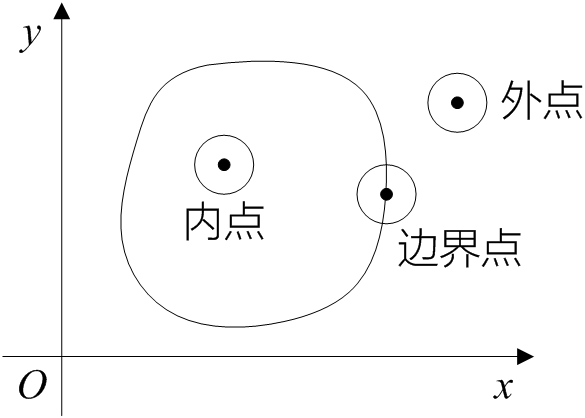
\includegraphics[height=3cm]{6.1.png}
\end{figure}

若$D$中每一个聚点都属于$D$,则称$D$为{\bf 闭集}。
若$D$中每个点都只是内点,称$D$为{\bf 开集}。
若开集$D$中任何两点均可用一条折线相连,则称为{\bf 连通的开集}或{\bf 开区域}。
开区域连同其边界称为{\bf 闭区域}。
对于点集$D$,若存在$M>0$,使得中任意两点的距离都小于$M$,称$D$为{\bf 有界区域},否则称为{\bf 无界区域}。
\end{definition}

这里,通过邻域的概念完整地定义了内点和外点,同时定义了边界点。
注意邻域概念的运用,对于内点外点,强调存在性,对于边界点,强调任一性。

最终要定义的是开区域和闭区域,类似一元函数中的开区间和闭区间,为此,需要首先定义各类点的概念和开集、闭集。

%============================================================
\subsection{二元数量值函数和二元向量值函数}

\begin{definition}[二元数量值函数]
设$D$为$\mathbb{R} ^2$的一个非空子集,$f$为$D\mapsto \mathbb{R} $的一个映射,对于$D$中的每一个矢量$\boldsymbol{p}$,$\mathbb{R} $中都有唯一的实数$z$与之对应,则称$f$为定义在$D$上的{\bf 二元数量值函数},也称{\bf 二元函数},写作:
\[
z=f\left( \boldsymbol{p} \right) \quad \boldsymbol{p}\in D
\]
其中$\boldsymbol{p}$称为{\bf 自变量},$z$称为{\bf 因变量},$D$称为{\bf 定义域}。
\end{definition}

二元数量值函数描述的是一个有序实数对到一个实数的映射:
\[
f:\boldsymbol{p}\mapsto z
\]
几何上可以用{\it xyz}直角坐标系描述。
$\boldsymbol{p}$表示平面{\it xy}平面上的点,$z$表示{\it z}轴上的值,$z=f\left( \boldsymbol{p} \right) $表示三维空间内的一个曲面。

\begin{definition}[二元向量值函数]
设$D$为$\mathbb{R} ^2$的一个非空子集,$\boldsymbol{f}$为$D\mapsto \mathbb{R} $的一个映射,对于$D$中的每一个矢量$\boldsymbol{p}$,$\mathbb{R} ^2$中都有唯一的实数$\boldsymbol{z}$与之对应,则称$\boldsymbol{f}$为定义在$D$上的{\bf 二元向量值函数},写作:
\[
\boldsymbol{z}=\boldsymbol{f}\left( \boldsymbol{p} \right) =\left( \begin{array}{c}
	P\left( \boldsymbol{p} \right)\\
	Q\left( \boldsymbol{p} \right)\\
\end{array} \right) \qquad \boldsymbol{p}\in D
\]
其中$\boldsymbol{p}$称为{\bf 自变量},$\boldsymbol{z}$称为{\bf 因变量},$D$称为{\bf 定义域},$P,Q$为$\boldsymbol{f}$对应的两个二元数量值函数。
\end{definition}

二元向量值函数描述的是一个有序实数到另一个有序实数对的映射:
\[
\boldsymbol{f}:\boldsymbol{p}\mapsto \boldsymbol{z}
\]
几何上比较难描述。

同样,可定义三维的向量值函数:
\[
\boldsymbol{z}=\boldsymbol{f}\left( \boldsymbol{p} \right) =\left( \begin{array}{c}
	P\left( \boldsymbol{p} \right)\\
	Q\left( \boldsymbol{p} \right)\\
	R\left( \boldsymbol{p} \right)\\
\end{array} \right) \qquad \boldsymbol{p}\in \mathbb{R} ^3
\]

%============================================================
\subsection{还是要光滑的}

一元函数微积分中,我们贯穿始终地考察光滑的曲线,二元函数也是一样。

学习二元函数微积分,我们可以将其与三维空间对应起来,用三维空间中的面和线,从几何角度理解二元函数微积分。
二元函数中我们喜欢的是光滑的面和线,同样需要对光滑进行定义。




